\documentclass[t]{beamer}
\usetheme[progressbar=frametitle]{metropolis}
\usepackage{appendixnumberbeamer}

\usepackage{booktabs}
\usepackage[scale=2]{ccicons}

\usepackage{graphics,graphicx,amssymb,amsmath,pgf,comment,hyperref}
%\usepackage[xcolor=pst]{pstricks}
\usepackage{array}
\usepackage{pgfshade}
\usepackage[round]{natbib}
\usepackage[absolute,overlay]{textpos}
\usepackage{pifont}
\usepackage{dcolumn}
\usepackage{textpos}
\usepackage{color}					
\usepackage{xcolor,colortbl}
\usepackage{tikz}
\usepackage{bbm}
\usepackage{curves}
\usepackage{mathtools}
\usetikzlibrary{snakes,arrows,positioning}
\def\augie{\fontencoding{T1}\fontfamily{augie}\selectfont}

\usepackage{pgfplots}
\usepgfplotslibrary{dateplot}

\usepackage{xspace}
\newcommand{\themename}{\textbf{\textsc{metropolis}}\xspace}

\setbeamertemplate{caption}{\raggedright\insertcaption\par}
\usetikzlibrary{calc,decorations.pathmorphing,patterns}
\pgfdeclaredecoration{penciline}{initial}{
    \state{initial}[width=+\pgfdecoratedinputsegmentremainingdistance,
    auto corner on length=1mm,]{
        \pgfpathcurveto%
        {% From
            \pgfqpoint{\pgfdecoratedinputsegmentremainingdistance}
                      {\pgfdecorationsegmentamplitude}
        }
        {%  Control 1
        \pgfmathrand
        \pgfpointadd{\pgfqpoint{\pgfdecoratedinputsegmentremainingdistance}{0pt}}
                    {\pgfqpoint{-\pgfdecorationsegmentaspect
                     \pgfdecoratedinputsegmentremainingdistance}%
                               {\pgfmathresult\pgfdecorationsegmentamplitude}
                    }
        }
        {%TO
        \pgfpointadd{\pgfpointdecoratedinputsegmentlast}{\pgfpoint{1pt}{1pt}}
        }
    }
    \state{final}{}
}


\title{Physician Behaviors and Hospital Influence}
\date{Emory University}
\author{Haizhen Lin \& \textbf{Ian McCarthy} \& Michael Richards}
\institute{October 29, 2018}

\begin{document}

\maketitle

\section{Background}

\begin{frame}{Physician Agency}
    \only<1>{
    Physician with decision-making authority for treatment
    \begin{itemize}
        \item Information asymmetry (what's wrong and how to fix it)
        \item Regulatory restrictions (I can't prescribe to or operate on myself)
    \end{itemize}
    }
    \only<2->{
    Differential financial incentives between physician and hospital
    \begin{itemize}
        \item More procedures $=$ more revenue, but location of procedure may matter to hospital
        \item Hospital wants less cost with fixed payment, but physician dictates resource use
    \end{itemize}
    }
    \onslide<3->{
    $\longrightarrow$ Incentives for hospitals to try to influence physician behaviors
    \vspace{.25in}
    }
    \onslide<4->{
    Most direct way to influence physician behavior is by purchasing the physician practice
    }
\end{frame}

\begin{frame}{How are hospitals and physicians related?}
    \only<1>{
        \begin{enumerate}
            \item ``Traditional'' private practice with admitting privileges
            \item Administrative support with or without admitting restrictions
            \item Practice owned by hospital or hospital system
        \end{enumerate}
    }
    \only<2>{
        \begin{figure}
            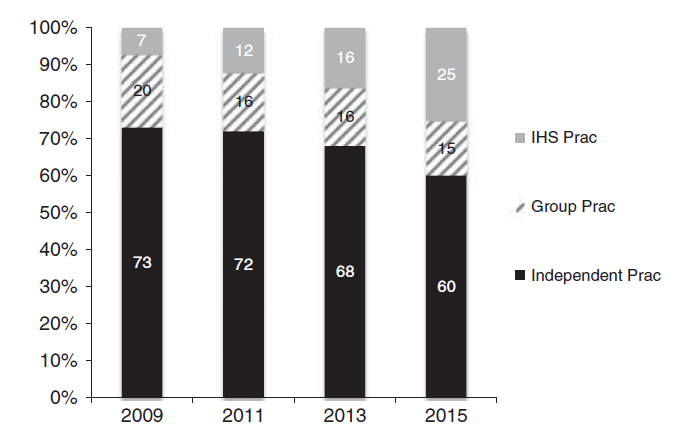
\includegraphics[height=2.4in,keepaspectratio]{Richardsetal.png}
            \caption{Richards \textit{et al.}, Medical Care, 2016}
        \end{figure}
    }
    \only<3>{
        \begin{figure}
            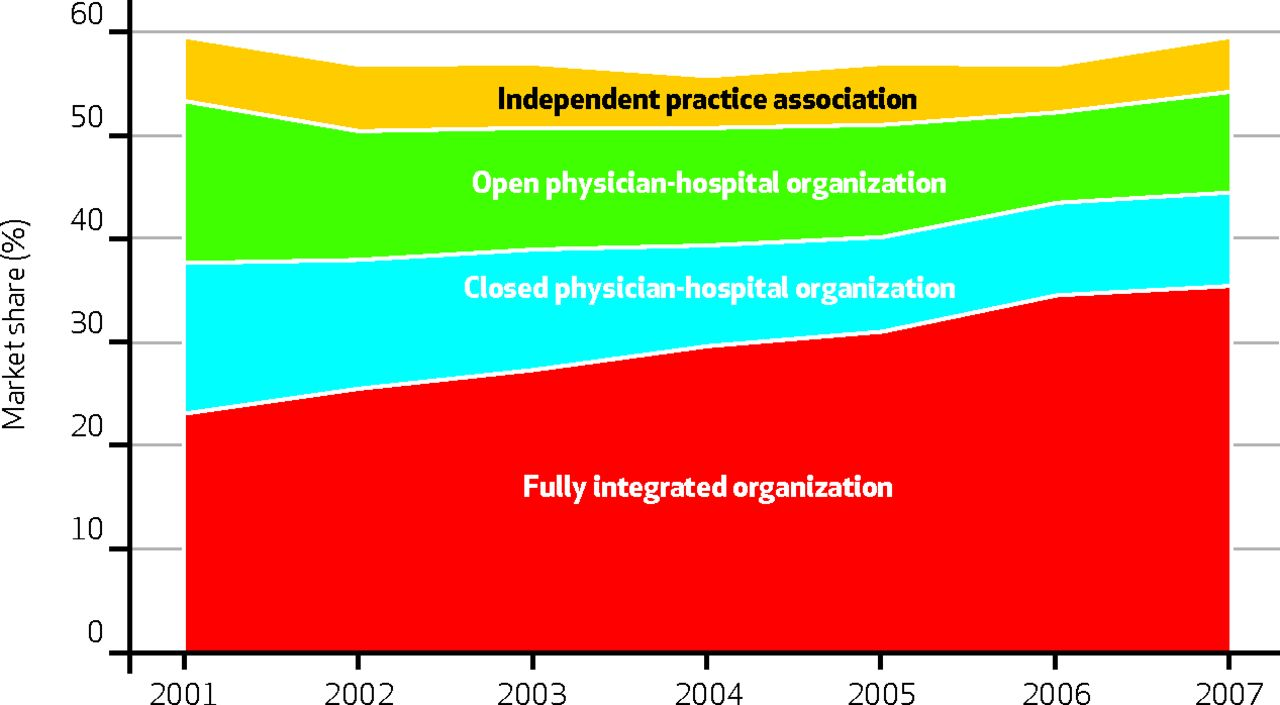
\includegraphics[height=2.3in,keepaspectratio]{Bakeretal.jpg}
            \caption{Baker, Bundorf, and Kessler, Health Affairs, 2014}
        \end{figure}
    }
\end{frame}

\begin{frame}{Why would a physician practice integrate?}
    \only<1>{
        \metroset{block=fill}
        \begin{block}{Financial security}
            \begin{itemize}
                \item Salaried arrangement
                \item Potential RVU incentives
            \end{itemize}
        \end{block}
    }

    \only<2>{
        \metroset{block=fill}
        \begin{block}{Reduce administrative burden (maybe)}
            \begin{itemize}
                \item Billing and insurance approvals
                \item Electronic Health Records
                \item Data collection/reporting
            \end{itemize}
        \end{block}
    }
\end{frame}

\begin{frame}{What do we expect from integration?}
    \begin{itemize}
        \item Hospitals claim efficiency gains, reduced fragmentation, increased coordination, etc.
        \item Financial incentives for cost increases and decreases
        \begin{itemize}
            \item[--] Lower costs with fixed payment 
            \item[--] Substituting locations of care more efficiently
            \item[--] Spillovers from private insurance
            \item[--] More resources due to pay-for-performance
        \end{itemize}
    \end{itemize}
\end{frame}

\section{Theoretical Framework}
\begin{frame}{Physician Agency}
    \only<1->{
    Observed care at time $t$ is
    \begin{equation*}
        y_{ijk} = \arg \max_{y}  \theta_{u} \tilde{u} \left(y; \Gamma_{j}, \kappa_{i} \right) + \theta_{\pi} \pi \left(y; \Gamma_{k}, \Gamma_{j} \right).
    \end{equation*}
    }
    \only<2->{
         Assuming:
         \begin{enumerate}
            \item<3-> $\tilde{u}$ is additively separable in $i$ and $(j,k)$
            \item<4-> maximizing levels of $y$ for $\tilde{u}$ and $\pi$ are linear in $y$
         \end{enumerate}
    }
    \only<5->{
    \begin{equation*}
        y_{ijk} = \alpha_{i} + x_{i}\beta + \Gamma_{jk} + \epsilon_{ijk}
    \end{equation*}
    }
\end{frame}

\begin{frame}{Estimation Strategy}
    \only<1-3>{
    Suggests two-step estimation strategy:
    \begin{enumerate}
        \item<2-> Estimate $y_{ijk} = \alpha_{i} + x_{i}\beta + \Gamma_{jk} + \epsilon_{ijk}$ at patient level (separately by year)
        \item<3-> Estimate $\hat{\Gamma}_{jkt} = \gamma_{j} + \gamma_{k} + \tau_{t} + z_{jkt}\delta + \eta_{jkt}$ with physician-hospital panel
    \end{enumerate}
    }
    \only<4>{
    \begin{itemize}
        \item Draws from ``match values'' in labor literature (Abowd \textit{et al.}, 2002; Card \textit{et al.}, 2013, QJE )
        \item Exploits variation across inpatient stays and splits the separation of match value into two steps
        \item Identifies effects on match value from within-physician variation across hospitals (e.g., patient movers in Finkelstein \textit{et al.}, 2016, QJE)
    \end{itemize}
    }
\end{frame}


\section{Data}
\begin{frame}{Data Sources}
    \begin{itemize}
        \item CMS: 100\% inpatient Medicare claims data (2008-2015)
        \item SK\&A: Hospital ownership of physician practices
        \item AHA, HCRIS, POS: Hospital characteristics
        \item Annual IPPS Impact Files: Hospital cost-to-charge ratios (CCR)
        \item ACS: County-level demographics, education, income, and employment
    \end{itemize}
\end{frame}

\begin{frame}{Sample Construction}
    \begin{itemize}
        \item<1-> Planned inpatient stays (elective admissions initiated by a physician, clinic, or HMO referral) and outpatient procedures with observed NPI for the operating physician
        \item<2-> Drop physicians operating in hospitals more than 120 miles from primary office or outside of contiguous U.S.
        \item<3-> Drop physicians with NPIs not matched in the SK\&A data
        \item<4-> Drop lowest/highest 1\% of charges and patients $<$ 65 years old
    \end{itemize}
  \uncover<5->{ $\longrightarrow$ 518,398 unique observations at the physician/hospital/year \\
   $\longrightarrow$ 7.5mm inpatient stays (47\% of total) and 24mm outpatient procedures}
\end{frame}



\section{Estimation of Match Values}
\begin{frame}{Specification}
    \only<1>{
    Two-step estimation strategy:
    \begin{enumerate}
        \item Estimate $y_{ijk} = \alpha_{i} + x_{i}\beta + \Gamma_{jk} + \epsilon_{ijk}$ at patient level (separately by year)
        \item Estimate $\hat{\Gamma}_{jkt} = \gamma_{j} + \gamma_{k} + \tau_{t} + z_{jkt}\delta + \eta_{jkt}$ with physician-hospital panel
    \end{enumerate}
    }
    \only<2>{
    \begin{equation*}
        y_{ijk} = \alpha_{i} + x_{i}\beta + \Gamma_{jk} + \epsilon_{ijk},
    \end{equation*}
    }
\end{frame}

\begin{frame}{Outcomes}
    \begin{equation*}
        \textcolor{red}{y_{ijk}} = \alpha_{i} + x_{i}\beta + \Gamma_{jk} + \epsilon_{ijk},
    \end{equation*}

    \begin{itemize}
        \item Total inpatient and outpatient Medicare payments
        \item Total inpatient and outpatient hospital costs (from cost-to-charge ratios)
        \item Inpatient hospital costs
        \item Inpatient length of stay
        \item Outpatient hospital costs
    \end{itemize}
\end{frame}


\begin{frame}{Independent Variables}
    \begin{equation*}
        y_{ijk} = \textcolor{red}{\alpha_{i}} + x_{i}\beta + \Gamma_{jk} + \epsilon_{ijk},
    \end{equation*}

    \begin{itemize}
        \item Quartiles of total ``other'' Medicare payments and procedures
        \item Covers 2008 through 2015 period
        \item Beneficiary-specific measure of ``utilization''
    \end{itemize}
\end{frame}

\begin{frame}{Independent Variables}
    \begin{equation*}
        y_{ijk} = \alpha_{i} + \textcolor{red}{x_{i}}\beta + \Gamma_{jk} + \epsilon_{ijk},
    \end{equation*}

    \begin{itemize}
        \item Age, gender, race
        \item Indicators for ICD9 diagnosis code groups (18 diagnosis groups per variable plus missing group)
        \item Indicators for primary DRGs (with at least 1000 observations in a given year)
        \item Minor differences between total, inpatient, and outpatient specifications
    \end{itemize}
\end{frame}

\begin{frame}{Summary of Match Values}
    \only<1>{
        \metroset{block=fill}
        \begin{block}{1. Calculate Cost Differential}
            Apply minimum cost physician-hospital combination to all of physician $j$'s patients:
            \begin{align*}
                \Delta_{k} y_{ij} &= \hat{y}_{ijk} - \hat{y}_{ij\underbar{k}} \nonumber \\
                   &= \hat{\alpha}_{i} + x_{i}\hat{\beta} + \hat{\Gamma}_{jk} - \hat{\alpha}_{i} - x_{i}\hat{\beta} - \min \left\{\Gamma_{j1},...,\Gamma_{jK} \right\} \nonumber \\
                   &= \hat{\Gamma}_{jk} - \min \left\{\Gamma_{j1},...,\Gamma_{jK} \right\}.
            \end{align*}
        \end{block}
    }
    \only<2>{
        \metroset{block=fill}
        \begin{block}{2. Summarize}
            \begin{itemize}
                \item Total cost differential for each physician
                \item Limit to pairs with 5 or more procedures
                \item Limit to physicians with 2 or more hospitals in a year
                \item Present interquartile range and mean
            \end{itemize}
        \end{block}
    }

\end{frame}

\begin{frame}{Within-physician Variation in Costs}
    \begin{figure}
        \centering
        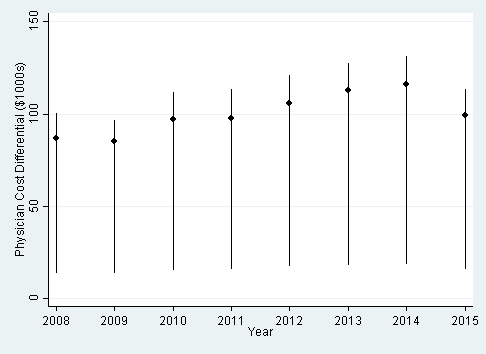
\includegraphics[height=2.5in,width=5in,keepaspectratio]{PhySave_Graph}
    \end{figure}
\end{frame}

\begin{frame}{Within-hospital Variation in Costs}
    \begin{figure}
        \centering
        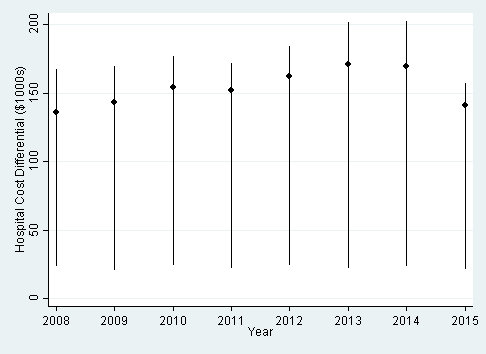
\includegraphics[height=2.5in,width=5in,keepaspectratio]{HospSave_Graph_DRG}
    \end{figure}
\end{frame}


\section{Estimation of Hospital Influence}
\begin{frame}{Specification}
    \only<1>{
    Two-step estimation strategy:
    \begin{enumerate}
        \item Estimate $y_{ijk} = \alpha_{i} + x_{i}\beta + \Gamma_{jk} + \epsilon_{ijk}$ at patient level (separately by year)
        \item Estimate $\hat{\Gamma}_{jkt} = \gamma_{j} + \gamma_{k} + \tau_{t} + z_{jkt}\delta + \eta_{jkt}$ with physician-hospital panel
    \end{enumerate}
    }
    \only<2>{
    \begin{equation*}
        \hat{\Gamma}_{jkt} = \gamma_{j} + \gamma_{k} + \tau_{t} + z_{jkt}\delta + \eta_{jkt},
    \end{equation*}
    }
\end{frame}

\begin{frame}{Main Outcomes}
    \begin{equation*}
        \textcolor{red}{\hat{\Gamma}_{jkt}} = \gamma_{j} + \gamma_{k} + \tau_{t} + z_{jkt}\delta + \eta_{jkt},
    \end{equation*}

    \begin{table}[htb!]
    \centering
    \footnotesize
    \centerline{
    \begin{tabular}{l|rrrrr|r}
        & 2008  & 2012 & 2013 & 2014 & 2015 & Overall \\
        \hline
Total Payments &      6446.6         &      7405.5         &      7753.0         &      8137.8         &      8282.3         &      7329.6         \\
            &    (5459.4)         &    (6396.5)         &    (6574.1)         &    (6664.7)         &    (6851.9)         &    (6226.6)         \onslide<2->{\\
Total Costs &      8473.5         &     10292.2         &     10725.9         &     11164.3         &     11477.0         &      9950.4         \\
            &    (6833.6)         &    (8180.3)         &    (8424.7)         &    (8769.9)         &    (8934.3)         &    (8001.9)         \onslide<3->{\\
Inpatient Costs &     13655.2         &     16958.0         &     17711.2         &     18366.9         &     18947.3         &     16280.6         \\
            &    (7751.8)         &    (9407.1)         &    (9612.3)         &    (9997.2)         &   (10460.7)         &    (9281.9)         \onslide<4->{\\
Inpatient LOS &       5.984         &       6.021         &       6.002         &       6.062         &       6.031         &       5.960         \\
            &     (2.427)         &     (2.493)         &     (2.494)         &     (2.513)         &     (2.613)         &     (2.449)         \onslide<5->{\\
Outpatient Costs &      3006.7         &      3805.5         &      4013.6         &      4189.6         &      4433.9         &      3698.7         \\
            &    (2135.0)         &    (2781.5)         &    (2925.1)         &    (3095.8)         &    (3275.4)         &    (2758.9)         }}}}\\
    \end{tabular}}
    \end{table}

\end{frame}


\begin{frame}{Independent Variables}
    \begin{equation*}
        \hat{\Gamma}_{jkt} = \gamma_{j} + \gamma_{k} + \tau_{t} + \textcolor{red}{z_{jkt}}\delta + \eta_{jkt},
    \end{equation*}

    \begin{table}[htb!]
    \centering
    \footnotesize
    \centerline{
    \begin{tabular}{l|rrrrr|r}
        & 2008  & 2012 & 2013 & 2014 & 2015 & Overall \\
        \hline
Integrated       &       0.130         &       0.206         &       0.233         &       0.255         &       0.332         &       0.196         \\
                 &     (0.336)         &     (0.404)         &     (0.422)         &     (0.436)         &     (0.471)         &     (0.397)         \onslide<2->{\\
Physician FTE       &       24.23         &       28.59         &       31.14         &       31.74         &       33.13         &       28.43         \\
                    &     (99.28)         &     (109.8)         &     (120.5)         &     (120.0)         &     (119.5)         &     (110.9)         \onslide<3->{\\
Resident FTE        &       25.77         &       28.45         &       29.13         &       30.69         &       30.97         &       28.08         \\
                    &     (108.2)         &     (120.4)         &     (121.4)         &     (125.9)         &     (127.8)         &     (117.8)         \onslide<4->{\\
Nurse FTE           &       340.8         &       365.7         &       369.1         &       384.9         &       402.7         &       364.8         \\
                    &     (446.8)         &     (487.8)         &     (494.8)         &     (519.1)         &     (550.7)         &     (487.3)         \onslide<5->{\\
Other FTE           &       749.9         &       763.0         &       761.8         &       776.4         &       806.0         &       762.8         \\
                    &     (975.5)         &    (1032.4)         &    (1076.2)         &    (1101.5)         &    (1157.2)         &    (1037.4)         \onslide<6->{\\
Beds (100s)         &       1.980         &       1.967         &       1.958         &       1.982         &       2.009         &       1.976         \\
                    &     (2.160)         &     (2.142)         &     (2.137)         &     (2.172)         &     (2.235)         &     (2.154)         }}}}}\\
    \end{tabular}}
    \end{table}

\end{frame}

\begin{frame}{Independent Variables}
    \begin{equation*}
        \hat{\Gamma}_{jkt} = \gamma_{j} + \gamma_{k} + \tau_{t} + \textcolor{red}{z_{jkt}}\delta + \eta_{jkt},
    \end{equation*}

    \begin{table}[htb!]
    \centering
    \footnotesize
    \centerline{
    \begin{tabular}{l|rrrrr|r}
        & 2008  & 2012 & 2013 & 2014 & 2015 & Overall \\
        \hline
Practice Size&       13.73         &       17.31         &       17.31         &       17.82         &       18.41         &       16.10         \\
             &     (32.10)         &     (30.70)         &     (29.28)         &     (28.46)         &     (28.02)         &     (30.05)         \onslide<2->{\\
Experience   &       22.55         &       23.00         &       23.94         &       23.65         &       24.77         &       23.17         \\
             &     (6.496)         &     (6.703)         &     (6.950)         &     (6.902)         &     (6.989)         &     (6.746)         \onslide<3->{\\
\% Multi-Specialty &       0.249         &       0.248         &       0.266         &       0.284         &       0.344         &       0.264         \\
\% with Surgery &       0.452         &       0.501         &       0.507         &       0.508         &       0.454         &       0.480         }}\\
    \end{tabular}}
    \end{table}

\end{frame}

\begin{frame}{Estimated Effects of Vertical Integration}
    \vspace{0.75in}
    \begin{table}[htb!]
    \centering
    \centerline{
    \begin{tabular}{l|rr}
        Outcome & Estimate & St. Error \\
        \hline\hline \onslide<2->{\vspace{-.1in}\\
        Total Medicare Payments & 72.68** & (33.88)  \onslide<3->{\\
        Total Hospital Costs & 140.39***  & (45.36) \onslide<4->{\\
        Inpatient Hospital Costs & 264.48*** & (54.71) \onslide<5->{\\
        Inpatient Length of Stay & -0.015 & (0.019) \onslide<6->{\\
        Outpatient Hospital Costs & -48.94** & (20.38) }}}}}\\
        \hline
        \multicolumn{3}{l}{* p-value $<$0.1, ** p-value $<$0.05, *** p-value $<$0.01}
    \end{tabular}}
    \end{table}
\end{frame}

\begin{frame}{Threats to Identification and Interpretation}
    Estimator is effectively a two-way fixed effects DD with time varying treatment
    \only<2>{
        \metroset{block=fill}
        \begin{block}{Potential Problems}
            \begin{enumerate}
                \item Vertical integration due to time-varying unobservables \& outcomes
                \item Weighted average of all 2$\times$2 DD estimates, with some potentially negative weights
            \end{enumerate}
        \end{block}
    }
\end{frame}

\begin{frame}{Event Study: Total Medicare Payments}
    \begin{figure}
        \centering
        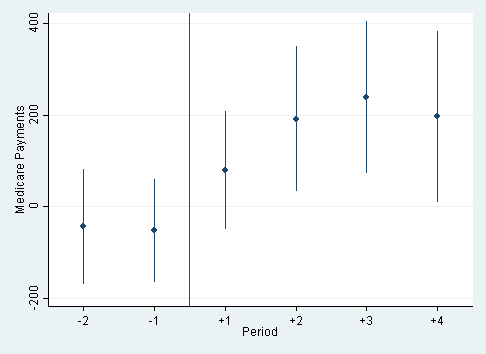
\includegraphics[height=2.5in,width=5in,keepaspectratio]{EventPay_All_2011}
    \end{figure}
\end{frame}

\begin{frame}{Event Study: Total Hospital Costs}
    \begin{figure}
        \centering
        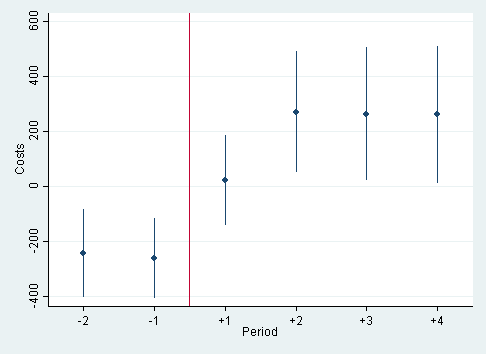
\includegraphics[height=2.5in,width=5in,keepaspectratio]{EventCharge_All_2011}
    \end{figure}
\end{frame}

\begin{frame}{Takeaways}
    \label{back}
    \begin{itemize}
        \item Evidence of increase in payments and costs
        \item Evidence consistent with common trends assumption for Medicare payments
        \item Some concern about common trends for costs
    \end{itemize}
    \vspace{1in}
    \onslide<2->{
    \footnotesize
    \hyperlink{ivs}{Thoughts on an Instrument}
    \normalsize
    }


\end{frame}

\section{Allocation of Procedures and Patients}
\begin{frame}{Other Effects}
    Other ways integration posited to affect physician behavior:
    \begin{itemize}
        \item More procedures overall (not per patient)
        \item Reallocating procedures from other hospitals
        \item Reallocating procedures across inpatient and outpatient settings
    \end{itemize}
\end{frame}

\begin{frame}{Results on Other Outcomes}
    \vspace{.75in}
    \begin{table}[htb!]
    \centering
    \centerline{
    \begin{tabular}{l|rr}
        Outcome & Estimate & St. Error \\
        \hline\hline \onslide<2->{\vspace{-.1in}\\
        Physician's inpatient share & 0.065*** & (0.003) \onslide<3->{\\
        Physician's outpatient share & 0.046***  & (0.003) \onslide<4->{\\
        Total patients & 6.070*** & (0.508) \onslide<5->{\\
        Inpatient procedures & 0.738*** & (0.162) \onslide<6->{\\
        Outpatient procedures & 8.367*** & (1.028) }}}}}\\
        \hline
        \multicolumn{3}{l}{* p-value $<$0.1, ** p-value $<$0.05, *** p-value $<$0.01}
    \end{tabular}}
    \end{table}
\end{frame}

\begin{frame}{Summary of Results}
    \only<1>{
        \metroset{block=fill}
        \begin{block}{Effects per Patient}
            \begin{itemize}
                \item Increase in Medicare payments and hospital costs
                \item Small effects per patient but meaningful effects in scope of cost reduction efforts
                \item Extrapolates to \$47 and \$91 million per year (about 0.17\% of observed Medicare spending)
            \end{itemize}
        \end{block}
    }

    \only<2>{
        \metroset{block=fill}
        \begin{block}{Sensitivity}
           \begin{itemize}
                \item Calculation of 2$\times$2 DD weights suggests relatively small portion of negative weights
                \item Event study consistent with common trends for Medicare payments but not for hospital costs
                \item As falsification test, no effects on payments or DRG weights per inpatient stay
            \end{itemize}
        \end{block}
    }

    \only<3>{
        \metroset{block=fill}
        \begin{block}{Effects on Total Patients and Allocation of Procedures}
           \begin{itemize}
                \item More procedures going to acquiring hospital
                \item New procedures predominantly coming from outpatient side (8 new outpatient procedures versus 1 inpatient)
            \end{itemize}
        \end{block}
    }
\end{frame}

\section*{Thank You}

\appendix
\begin{frame}{Endogeneity of physician-hospital integration}
    \label{ivs}
    \only<1>{
        Integration could be driven by:
        \begin{itemize}
            \item Existing physician behaviors
            \item Unobserved, time-varying practice characteristics
        \end{itemize}
    }
    \only<2>{
        \metroset{block=fill}
        \begin{block}{1. Set of possible physician-hospital pairs}
            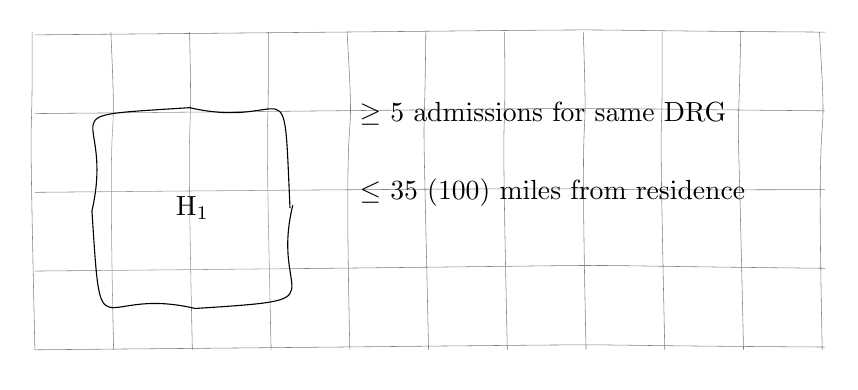
\begin{tikzpicture}[decoration=penciline, decorate]
                \draw[decorate,style=help lines] (0,0) grid[step=1cm] (10,4);

                % Patient 1
                \node[decorate,draw,inner sep=.7cm,fill=white,fill opacity=.2,text opacity=1,circle] (a) at (2,1.8) {$\text{H}_{1}$};

                \node[right] at (4,3) {$\geq$ 5 admissions for same DRG};
                \node[right] at (4,2) {$\leq$ 35 (100) miles from residence};
            \end{tikzpicture}
        \end{block}
    }
    \only<3>{
        \metroset{block=fill}
        \begin{block}{1. Set of possible physician-hospital pairs}
            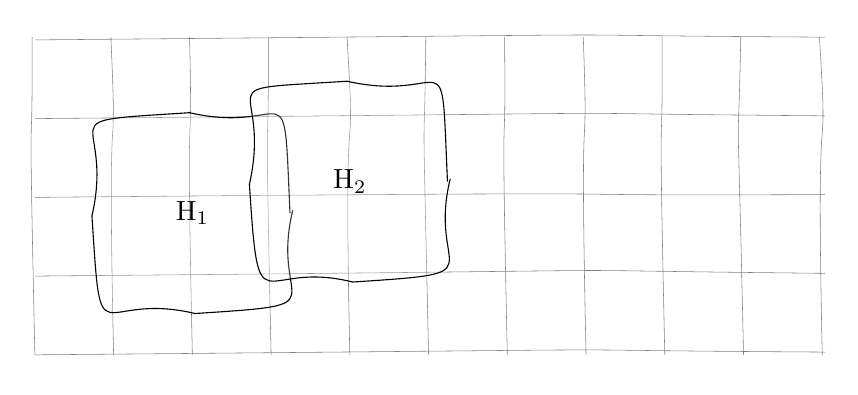
\begin{tikzpicture}[decoration=penciline, decorate]
                \draw[decorate,style=help lines] (0,0) grid[step=1cm] (10,4);

                % Patient 1
                \node[decorate,draw,inner sep=.7cm,fill=white,fill opacity=.2,text opacity=1,circle] (a) at (2,1.8) {$\text{H}_{1}$};

                % Patient 2
                \node[decorate,draw,inner sep=.7cm,fill=white,fill opacity=.2,text opacity=1,circle] (a) at (4,2.2) {$\text{H}_{2}$};

            \end{tikzpicture}
        \end{block}
    }
    \only<4>{
        \metroset{block=fill}
        \begin{block}{1. Set of possible physician-hospital pairs}
            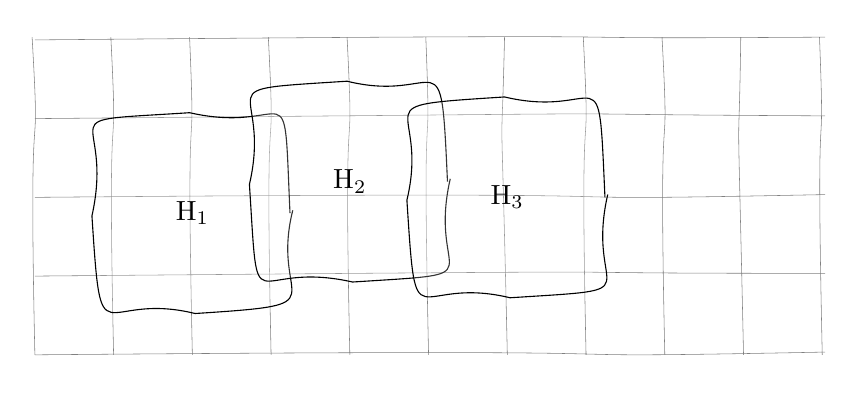
\begin{tikzpicture}[decoration=penciline, decorate]
                \draw[decorate,style=help lines] (0,0) grid[step=1cm] (10,4);

                % Patient 1
                \node[decorate,draw,inner sep=.7cm,fill=white,fill opacity=.2,text opacity=1,circle] (a) at (2,1.8) {$\text{H}_{1}$};

                % Patient 2
                \node[decorate,draw,inner sep=.7cm,fill=white,fill opacity=.2,text opacity=1,circle] (a) at (4,2.2) {$\text{H}_{2}$};

                % Patient 3
                \node[decorate,draw,inner sep=.7cm,fill=white,fill opacity=.2,text opacity=1,circle] (a) at (6,2) {$\text{H}_{3}$};

            \end{tikzpicture}
        \end{block}
    }
    \only<5>{
        \metroset{block=fill}
        \begin{block}{1. Set of possible physician-hospital pairs}
            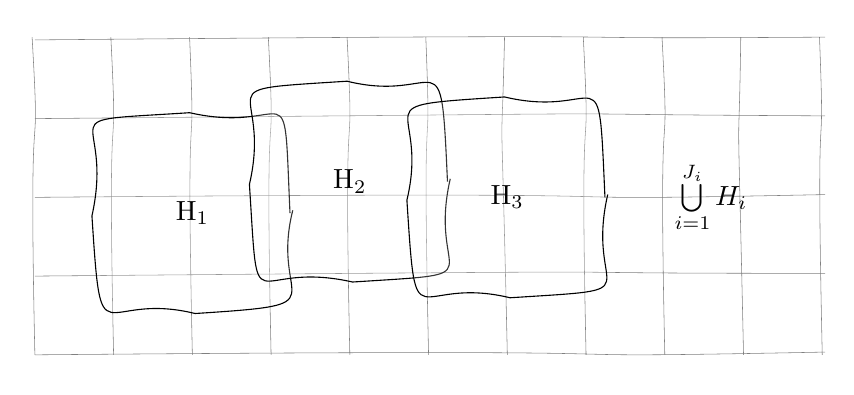
\begin{tikzpicture}[decoration=penciline, decorate]
                \draw[decorate,style=help lines] (0,0) grid[step=1cm] (10,4);

                % Patient 1
                \node[decorate,draw,inner sep=.7cm,fill=white,fill opacity=.2,text opacity=1,circle] (a) at (2,1.8) {$\text{H}_{1}$};

                % Patient 2
                \node[decorate,draw,inner sep=.7cm,fill=white,fill opacity=.2,text opacity=1,circle] (a) at (4,2.2) {$\text{H}_{2}$};

                % Patient 3
                \node[decorate,draw,inner sep=.7cm,fill=white,fill opacity=.2,text opacity=1,circle] (a) at (6,2) {$\text{H}_{3}$};

                \node[right] at (8,2) {$\bigcup\limits_{i=1}^{J_{i}} H_{i}$};
            \end{tikzpicture}
        \end{block}
    }
    \only<6>{
        \metroset{block=fill}
        \begin{block}{2. Estimate probability of integration (at practice level)}
            \begin{equation*}
                I_{pk} = \lambda z_{pk} + \omega_{pk}
            \end{equation*}
            \vspace{-.3in}
            \begin{itemize}
                \item Average choice set size
                \item Average differential distance (relative to nearest hospital)
                \item Differential distance interacted with hospital characteristics
            \end{itemize}
        \end{block}
    }
    \only<7>{
        \metroset{block=fill}
        \begin{block}{2. Estimate probability of integration}
            \begin{equation*}
                I_{pk} = \lambda z_{pk} + \omega_{pk}
            \end{equation*}
            \vspace{-.3in}
            \begin{itemize}
                \item Average choice set size
                \item Average differential distance (relative to nearest hospital)
                \item Differential distance interacted with hospital characteristics
            \end{itemize}
        \end{block}
        \begin{equation*}
            \hat{\Gamma}_{jkt} = \gamma_{j} + \gamma_{k} + \tau_{t} + \underbrace{I_{jkt}}_{\mathclap{\hat{I}_{jkt}=\text{Pr}(I_{jkt}=1)}} \delta_{1}  + \tilde{z}_{jkt}\delta_{2} + \eta_{jkt},
        \end{equation*}
        \hyperlink{back}{Back to presentation}
    }
\end{frame}

\end{document}






